\chapter{QFT en sistemas acelerados y espacio curvo}

\todo{Mejor meter subsecciones?}
\section{Efecto Unruh}

Una propiedad sorprendente de las teorías cuánticas de campos es que el estado de vacío
puede depender del observador.
Concretamente, el efecto Unruh establece que el vacío para un observador inercial,
visto por un observador con aceleración constante corresponde con un estado térmico a temperatura
\begin{equation}
  T_U=\frac{a}{2\pi k_B}.
\end{equation}

En la deducción del efecto Unruh estudiaremos un campo escalar sin masa $\phi(t,z)$ en un espacio de Minkowski
con una dimensión espacial $t$ y una dimensión espacial $z$.  
\todo{Argumentar por qué es válido usar esta teoría}
La ecuación que describe el campo es la ecuación de Klein-Gordon
\begin{equation}
  -\pdv[2]{\phi}{t}+\pdv[2]{\phi}{z}=0.
\end{equation}

La solución general de esta ecuación de ondas toma la forma
\begin{equation}
  \phi(x,t)=f(t-x)+g(t+x).
\end{equation}

Las funciones $f$ y $g$ representan dos ondas que se mueven a la velocidad de la luz en sentidos
opuestos. 
Hacemos el cambio de variable a coordenadas nulas
\begin{equation}
  U=t-z,   \qquad V=t+z.
\end{equation}

De este modo, la solución general se expresa como
\begin{equation}
  \phi(U,V)=\phi_U(U)+\phi_V(V).
\end{equation}

Nos interesa expandir la solución en términos de ondas armónicas
\begin{gather}
  \phi_\omega^U(U)=\frac{1}{\sqrt{4\pi\omega}} e^{-i\omega U},  \\
  \phi_\omega^V(V)=\frac{1}{\sqrt{4\pi\omega}} e^{-i\omega V}.
\end{gather}

Puesto que la solución $\phi_V$ está desacoplada de $\phi_U$, basta considerar $\phi_U$ ya que
el tratamiento de $\phi_V$ sería análogo.

La expansión del campo en modos es
\begin{equation}
\phi_U(U) = \int_0^\infty d\omega \qty[a_\omega^U \phi_\omega^\phi (U)+a_\omega^{U*} \phi_\omega^\phi (U)^*].
\end{equation}

El proceso de cuantización canónica consiste en reemplazar en valor del campo en cada
punto del espacio-tiempo $\phi(x,t)$, por un operador $\widehat \phi(x,t)$ que satisfará unas
relaciones de conmutación particulares. 
Esto significa que los coeficientes de la expansión de $\phi_U$ pasan a ser los operadores
$\widehat a_\omega^U$ y $\widehat a_\omega^{U\dagger}$ y por tanto
\begin{equation}
  \widehat \phi_U(U) = \int_0^\infty d\omega \qty[\widehat a_\omega^U\phi_\omega^\phi (U)+\widehat a_\omega^{U\dagger} \phi_\omega^\phi (U)^*].
\end{equation}

El operador $\widehat a_\omega^{U\dagger}$ se denomina operador creación, pues veremos que crea 
partículas de frecuencia $\omega$ y $\widehat a_\omega^U$ se conoce como operador destrucción porque
aniquila partículas de frecuencia $\omega$.
Las relaciones de conmutación que cumplen son
\begin{gather}
  [\widehat a_\omega^{U\dagger},\widehat a_{\omega'}^{U\dagger}]=[\widehat a_\omega^U,\widehat a_{\omega'}^U]=0, \\
  [\widehat a_\omega^U,\widehat a_{\omega'}^{U\dagger}]=\delta(\omega-\omega').
\end{gather}

Todavía no hemos especificado el espacio de Hilbert sobre el que actúa el operador del campo, el cual
se denota por $\mathcal H_\phi$. 
El estado del campo queda especificado descrito por un elemento de $\mathcal H_\phi$.
Como en este caso los modos $U$ y $V$ están desacoplados, podemos considerar independientemente el espacio
de Hilbert asociado a cada uno, $\mathcal H_U$ y $\mathcal H_V$.
El espacio de Hilbert del campo es el producto tensorial de ambos $\mathcal H_\phi=\mathcal H_U\otimes \mathcal H_V$.

%Construcción espacio de Fock
La base del espacio $\mathcal H_U$ se puede construir mediante la representación de Fock. 
Para ello, se define el estado de vacío $\ket{0_U}$, como el estado que no contiene ningún tipo
de partícula, por tanto
\begin{equation}
  a^U_\omega \ket{0_U} = 0.
\end{equation}

Donde omitimos el acento circunflejo de los operadores por comodidad.
Luego procedemos a crear estados con $n_i$ partículas de frecuencia $\omega_i$, mediante
aplicación repetida del operador creación $a_{\omega_i}^{U\dagger}$, con la normalización apropiada
\begin{equation}
  \ket{n_{1,\omega_1}, n_{2,\omega_2},\cdots,n_{N,\omega_N}} = \frac{1}{\sqrt{n_1!n_2!\cdots n_N!}}(a_{\omega_1}^{U\dagger})^{n_1}
  (a_{\omega_2}^{U\dagger})^{n_2}\cdots a_{\omega_N}^{U\dagger})^{n_N} \ket{0_U}.
\end{equation}

Los estados construidos son estados propios del operador número de partículas $N_{\omega_i}^U=a_{\omega_i}^{U\dagger}a_{\omega_i}^U$
con valor propio $n_i$.
La base de $\mathcal H_U$ se obtiene juntando los estados con un número arbitrario de partículas
de todas las frecuencias posibles.
\todo{La suma directa es no numerable, al tener que considerar todas las frecuencias?}
Formalmente, $\mathcal H_U$ es la completitud de la suma directa 
\todo{Rigor}
\begin{equation}
  \mathcal H_U = \oplus  .
\end{equation}

%Expansión en otra base. Transformación Bogoliubov. Vacío.
Supongamos que queremos expandir el campo en otra base de modos $u$
\begin{equation}
  \phi_\omega^u(U)=\frac{1}{\sqrt{4\pi\omega}}e^{-i\omega u(U)}, 
\end{equation}

entonces
\begin{equation}
  \phi_U(U) = \int_0^\infty d\omega [a_\omega^u \phi^u_\omega(U) +  a_\omega^{u*} \phi_\omega^u(U)^*].
\end{equation}

Expandiendo la nueva base en términos de la anterior
\begin{equation}
  \phi_\omega^u(U) = \int_0^\infty d\omega'\qty[ \alpha_{\omega\omega'} \phi_{\omega'}^U(U) 
  +\beta_{\omega\omega'} \phi_{\omega'}^U(U)^*].
\end{equation}

Los coeficientes $\alpha_{\omega\omega'}$ y $\beta_{\omega\omega'}$ se denominan coeficientes
de Bogoliubov y vienen dados por
\begin{gather}
  \alpha_{\omega\omega'} = -\frac{1}{2\pi}\sqrt{\frac{\omega'}{\omega}}\int_{-\infty}^\infty dU e^{-i(\omega u(U) -\omega' U)},\\
  \beta_{\omega\omega'} = -\frac{1}{2\pi}\sqrt{\frac{\omega'}{\omega}}\int_{-\infty}^\infty dU e^{-i(\omega u(U) +\omega' U)}.
\end{gather}

Cuantizando la teoría y formando el espacio de Fock, comprobamos que el vacío obtenido mediante
los modos $\phi^U_\omega (U)$, puede contener partículas asociadas a los modos $u$
si el coeficiente $\beta_{\omega\omega'}$ no es nulo
\begin{equation}
  \ev{0_U}{N_\omega^u}=\int_0^\infty d\omega' \abs{\beta_{\omega\omega'}}^2.
\end{equation}

Esto quiere decir que en una teoría cuántica de campos, el vacío depende de la base de modos
que se haya escogido antes de la cuantización.
\todo{En realidad la ambigüedad es el concepto de partícula}
La ambigüedad se puede resolver escogiendo el vacío que tenga la mínima energía.
En el espacio de Minkowski la energía está bien definida y coincide para todos los observadores
inerciales, al ser invariante de Lorentz.
Sin embargo, en un espacio-tiempo curvo el concepto de energía puede no estar bien definido
y por tanto no hay un estado de vacío privilegiado.
\todo{Tiene algún sentido el concepto de partícula en un espacio que no sea asintóticamente
plano o no estacionario?}

%Observadores acelerados
Con el fin de estudiar cuál es el vacío dado por un observador acelerado en un espacio de 
Minkowski, introducimos las coordenadas de Rindler $(\eta,\xi)$ definidas por
\begin{gather}
  t=\frac{1}{a} e^{a\xi} \sinh a\eta ,\\
  z=\frac{1}{a}e^{a\xi} \cosh a\eta,
\end{gather}
donde $\abs{t}<z$ y $a>0$.

Las coordenadas de Rindler solo cubren la región $\abs{t}<z$, denominada cuña derecha de Rindler.
De forma análoga, se puede cubrir la cuña izquierda de Rindler ($\abs{t}<-z$) mediante
las coordenadas $(\tilde \eta, \tilde \xi)$ dadas por
\begin{gather}
  t=-\frac{1}{a} e^{a\tilde \xi} \sinh a\tilde \eta \\
  z=-\frac{1}{a} e^{a\tilde \xi} \cosh a\tilde \eta.
\end{gather}

%Usar imagen libre, centrar
\begin{figure}[htb]
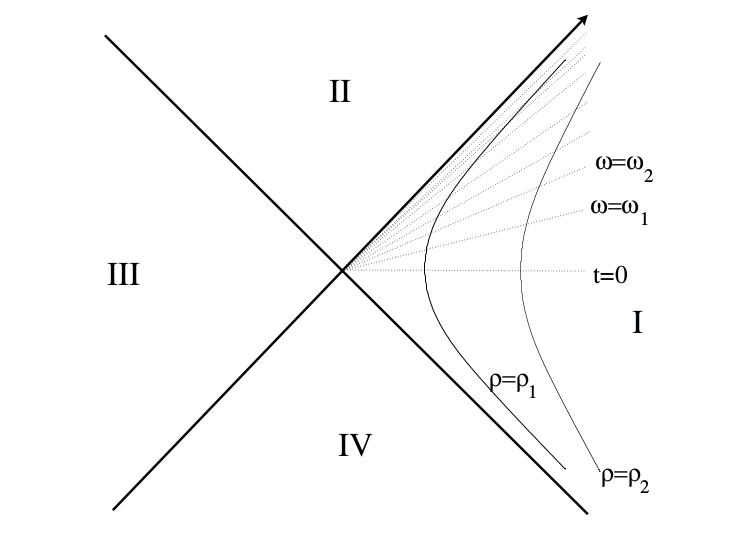
\includegraphics[width=0.8\textwidth]{rindler.png}\hfill
 \caption{Espacio de Minkowski en coordenadas de Rindler (usar imagen libre)
}                   
  \label{fig:rindler}
\end{figure}

Las trayectorias con $\eta=\eta_0$ constante corresponden con observadores que se mueven con
aceleración propia $ae^{-a\xi_0}$.
\todo{Pq $\xi_0=0$}
El tiempo propio que miden estos observadores es $\tau = e^{a\xi_0}\eta$.
Escogiendo apropiadamente el origen de coordenadas, un observador con aceleración constante
es tiene viene dado por $\eta=\tau$ y $\xi=0$.

Fijándonos en el diagrama de Rindler (figura \ref{fig:rindler}),
un observador con aceleración constante moviéndose a la derecha no puede percibir los 
efectos producidos  en III ni influir en II. 
Además, la información que le llegue de II será percibida como proveniente de un tiempo
infinitamente anterior, por lo que la recta $t=z$ define un horizonte de sucesos futuro y 
la recta $t=-z$ un horizonte de sucesos pasado.

Como el observador acelerado hacia la derecha desconoce el estado del campo en la 
cuña izquierda de Rindler, el estado que percibe no es puro, si no mixto.
La descripción de estados mixtos se realiza mediante una matriz de densidad, que al trazar
sobre los estados desconocidos conduce a que el vacío sea un estado térmico.
Con el fin de hacer la deducción explícita, partimos de la ecuación de Klein-Gordon en
coordenadas de Rindler para la cuña derecha
\begin{equation}
  -\pdv[2]{\phi}{\eta}+\pdv[2]{\phi}{\xi} = 0.
  \label{eq:kgr}
\end{equation}

Definiendo la coordenadas nulas de Rindler 
\begin{equation}
  \begin{gathered}
  u=\eta-\xi,\\
  v=\eta+\xi, 
  \end{gathered}
\end{equation}

la solución general de \ref{eq:kgr} es $\phi(u,v)=\phi_u(u)+\phi_v(v)$, que se expande en los
modos normales
\begin{equation}
  \begin{aligned}
    \phi^u_\omega(u) &=\frac{1}{\sqrt{4\pi\omega}}e^{-i\omega u},\\
    \phi^u_\omega(v) &=\frac{1}{\sqrt{4\pi\omega}}e^{-i\omega v}.
  \end{aligned}
\end{equation}

Aplicaríamos un tratamiento análogo a la cuña izquierda.

El campo propagándose hacia la derecha en coordenadas de Minkowski se expande como
\begin{equation}
  \begin{aligned}
    \phi_U(U)=&\int_0^\infty \Theta(-U)\qty[a^u_\omega \phi^u_\omega(u(U))+a_\omega^{u*}\phi_\omega^u(u(U))^*] \\
    &+\Theta(U)\qty[a^{\tilde u}_\omega \phi^{\tilde u}_\omega(\tilde u(U))+a_\omega^{\tilde u*}\phi_\omega^{\tilde u}(\tilde u(U))^*].
  \end{aligned}
\end{equation}

Donde $\Theta(U)$ es la función de Heaviside 
\begin{equation}
   \Theta(U)=
  \begin{cases}
    0\qquad \text{si }U<0 \\
    1\qquad \text{si }U>0
  \end{cases}
  .
\end{equation}

El cálculo de los coeficientes de Bogoliubov conduce a 
\todo{Tal vez separar}
\begin{equation}
  \begin{aligned}
    &\alpha_{\omega,\omega'}^{ u} = -\frac{e^{\frac{\pi\omega}{2 a}}}{2\pi a}\sqrt{\frac{\omega}{\omega'}}\qty(\frac{\omega'}{a})^{-i\omega/a}
    \Gamma(i\omega/a), \quad
    \beta_{\omega,\omega'}^{ u} = \frac{e^{-\frac{\pi\omega}{2 a}}}{2\pi a}\sqrt{\frac{\omega}{\omega'}}\qty(\frac{\omega'}{a})^{-i\omega/a}
    \Gamma(i\omega/a)\\
    &\alpha_{\omega,\omega'}^{\tilde u} = -\frac{e^{\frac{\pi\omega}{2 a}}}{2\pi a}\sqrt{\frac{\omega}{\omega'}}\qty(\frac{\omega'}{a})^{i\omega/a}
    \Gamma(-i\omega/a), \quad
    \beta_{\omega,\omega'}^{\tilde u} = \frac{e^{-\frac{\pi\omega}{2 a}}}{2\pi a}\sqrt{\frac{\omega}{\omega'}}\qty(\frac{\omega'}{a})^{i\omega/a} 
    \Gamma(-i\omega/a)
  \end{aligned}
\end{equation}

Por conveniencia, los modos de Unruh se definen como
\begin{equation}
  \begin{aligned}
    \phi^I_\omega(U)=\Theta(-U)\phi^u_\omega(u(U)) + e^{-\frac{\pi\omega}{a}}\Theta(U)\phi_\omega^{\tilde u}(\tilde u(U))^*,\\
    \phi^{II}_\omega(U)=\Theta(U)\phi^{\tilde u}_\omega(\tilde u(U)) + e^{-\frac{\pi\omega}{a}}\Theta(-U)\phi_\omega^{u}(u(U))^*.
  \end{aligned}
\end{equation}

La cuantización de los modos de Unruh conduce a los operadores creación y destrucción
\begin{equation}
  \begin{aligned}
    a_\omega^I = -2\sinh\frac{\pi\omega}{a}\int_0^\infty d\omega' \beta_{\omega\omega'}^{\tilde u} a_{\omega'}^U,\\
    a_\omega^{II} = -2\sinh\frac{\pi\omega}{a}\int_0^\infty d\omega' \beta_{\omega\omega'}^{u} a_{\omega'}^U.\\
  \end{aligned}
\end{equation}
 

\begin{equation}
  \ev{a_\omega^{u\dagger}a_\omega^u}{0_H} = \int_0^\infty d\omega'' \beta_{\omega\omega''}^u
  \beta_{\omega'\omega''}^{u*} = \frac{1}{e^{\frac{2\pi\omega}{a}}-1}\delta(\omega-\omega').
\end{equation}

\begin{equation}
  \phi_{n,\bar n}(\bar u)=\frac{1}{\sqrt{\Delta \omega}}\int_{n\Delta}^{(n+1)\Delta \omega} e^{i\frac{2\pi \bar n n}{\Delta \omega}}
  \phi_\omega(\bar u).
\end{equation}


\begin{equation}
  \ket{0_H} = \prod_{n,\bar n} \qty(\sum_{m=0}^\infty K_{nm} \ket{m_{n\bar n}}_u\otimes \ket{m_{n\bar n}}_{\bar u}).
\end{equation}

\begin{equation}
  K_{n,m+1}=e^{-\frac{\pi n\Delta \omega }{a}}K_{nm}.
\end{equation}

\begin{equation}
  \ket{0_H} = \prod_{n,\bar n} \qty(\sum_{m=0}^\infty e^{-\frac{\pi n\Delta \omega }{a}}K_{nm}\ket{m_{n\bar n}}_u\otimes \ket{m_{n\bar n}}_{\bar u}).
\end{equation}

\begin{equation}
  \ev{0_U}{N^u_{n,\bar n}} =
\end{equation}

\begin{equation}
  \rho 
\end{equation}

\section{Radiación de Hawking}
\todo{Obtenemos el resultado para observadores asintóticos}

%Introducción relatividad general. Métrica Schwarzschild


%Transformación de coordenadas. Ecuación de ondas. Modos Boulware.


%Propagación al pasado.





\todo{Cálculo Unruh en un BH por path integral}
El caso más sencillo de agujero negro es el agujero negro de Schwarzschild, que
describe una distribución de masa con simetría esférica y estática. La métrica asociada
es 
\begin{equation}
  ds^2= \qty(1-\frac{2MG}{r})dt^2-\qty(1-\frac{2MG}{r})^{-1}dr^2-r^2d\Omega^2.
\end{equation}

Observamos que en el radio de Schwarzschild $r_S=2MG$ la componente temporal de la 
métrica se anula mientras que la componente radial va a infinito.
Se denomina horizonte de sucesos a la esfera con radio $r_S$ centrada en $r=0$.

Para estudiar la física cerca del horizonte es más conveniente emplear las coordenadas
de Rindler. Para ello sustituimos la coordenada radial por la distancia propia hasta
el horizonte
\begin{equation}
  \rho(r)=\int_0^r dr' \sqrt{g_{rr}(r')}.
\end{equation}

La métrica se transforma en 
\begin{equation}
  ds^2=\qty(1-\frac{2MG}{r(\rho)})dt^2-d\rho^2-r(\rho)^2d\Omega^2.
\end{equation}

A distancias próximas al horizonte $r\approx r_S$, $\rho\approx 2\sqrt{2MG(r-2MG)}$
\begin{equation}
  ds^2\approx \rho^2\qty(\frac{dt}{4MG})^2 -d\rho^2-r(\rho)^2d\Omega^2.
\end{equation}

Cerca de la coordenada azimutal $\theta=0$, podemos reemplazar las coordenadas
angulares $\theta,\phi$ por las coordenadas cartesianas $x,y$. Definiendo
también un tiempo adimensional $\omega=t/(4MG)$ obtenemos la métrica de Rindler
\begin{equation}
  ds^2=\rho^2d\omega^2 -d\rho^2 -dx^2-dy^2.
\end{equation}

Esta métrica describe en realidad un espacio de Minkowski en coordenadas hiperbólicas.
Si escogemos la transformación
\begin{align}
  T&=\rho \sinh \omega, \\
  Z&=\rho \cosh \omega.
\end{align}
la métrica es
\begin{equation}
  ds^2=dT^2-dZ^2-dx^2-dy^2.
\end{equation}

Es conveniente definir un observador fijo para cada punto del espacio, llamado
FIDO. Estos observadores para mantenerse
en reposo dentro del campo gravitatorio necesitan una fuerza que los mantenga
en su sitio. Para los FREFOs, su aceleración es, para $\rho<<MG$ es aproximadamente $1/\rho$.

Si dividimos el espacio de Minkowski en cuatro regiones, el espacio de Rindler ocupa
la región I. Los FREFOs emplean el las coordenadas del (T,Z,x,y), mientras que
los FREFOS emplean $(\omega, \rho, x, y)$. El horizonte se sitúa en $T=Z=0$, o
en coordenadas de Rindler, $\rho=0$.
Gráficamente, se observa que una translación espacial de $\omega$ para un equivale
a un boost en el espacio de Minkowski.

Al espacio de Rindler solo le llega información de I y IV, pero la región II está 
desconectada causalmente por culpa del horizonte.
Además, un partícula que pase de IV a I será vista como proveniente del tiempo 
$\omega=-\infty$, por lo que se pueden interpretar como condiciones iniciales.

Estudiamos un campo escalar masivo cuántico $\xi$ en un espacio de Rindler.
La evolución temporal de un sistema cualquiera viene dada por un hamiltoniano. En el
espacio de Rindler la evolución en $\omega$ se determina mediante el hamiltoniano de
Rindler, cuya expresión en función del tensor energía-momento es
\begin{equation}
  H_R=\int_0^\infty d\rho dxdy \rho T^{00} (\rho, x, y).
\end{equation}

En el caso de un campo escalar masivo sometido a un potencial $V$, la densidad de energía
es
\begin{equation}
  T^{00}=\frac{\Pi^2}{2}+\frac{1}{2}\qty(\nabla \xi)^2+V(\xi).
\end{equation}

Entonces el hamiltoniano es
\begin{equation}
  H_R=\int_0^\infty d\rho dx_\perp \frac{\rho}{2}\qty(\Pi^2+\qty(\pdv{\xi}{\rho})^2+\qty(\pdv{\xi}{x_\perp})^2+2V(\xi)).
\end{equation}

Desde el punto de vista del espacio de Minkowski, $H_R$ es el generador de boosts en 
la dirección Z.

En una teoría cuántica, el hecho que haya correlación entre el campo para dos puntos
del espacio origina un fenómeno interesante en el espacio de Rindler. 
Hemos visto que la región III está desconectada de la región I, por lo que consideramos
al campo en cada región como subsistemas distintos. Pero debido a que el campo en I está
correlacionado con el campo III, están entrelazados entre sí.
Por esta razón, no podemos describir al campo en I como un sistema puro como una
matriz de densidad obtenida tomando la traza parcial en III de la matriz de densidad
del sistema completo.

En general, si el estado asociado a dos subsistemas A y B que no están interactuando 
es $\ket{\Psi}$, su matriz de densidad es
\begin{equation}
  \rho_{AB}=\ket{\Psi}\bra{\Psi}.
\end{equation}

La matriz de densidad que describe el sistema A es
\begin{equation}
  \rho_{A}=\Tr_B \rho_{AB}=\expval{\rho_{AB}}{\beta}.
\end{equation}
 
A cada matriz de densidad le corresponde la entropía de von Neumann
\begin{equation}
  S=-\Tr (\rho_A \ln \rho_A)=-\sum_j \rho_j \ln \rho_j.
\end{equation}

Donde $\rho_j$ son los valores propios de $\rho_A$.
Esta entropía se debe a que estamos perdiendo información al ignorar el subsistema $B$, que 
está entrelazado con $A$, por lo que también se denomina entropía de entrelazamiento.
La interpretación de $\rho_j$ es que estamos describiendo un sistema cuyo estado no 
conocemos, pero sabemos que a cada estado le corresponde una probabilidad $\rho_j$.

Por otro lado un sistema termodinámico en equilibrio a temperatura $\beta$ tiene 
asociado la matriz densidad 
\begin{equation}
  \rho=\frac{e^{-\beta H}}{\Tr e^{\beta H}}.
\end{equation}

Retomamos el campo escalar en un espacio de Rindler. 
Para $T=0$, los campos en cada punto forman un conjunto completo de observables que 
conmutan. Denominamos $\xi_L$ a los campos en $Z<0$ y $\xi_R$ si $Z>0$.
En teoría cuántica de campos, un estado se describe como una distribución que 
depende de los campos $\Psi[\xi]=\Psi[\xi_L,\xi_R]$.

Supondremos que $\Psi[\xi_L,\xi_R]$ está en el estado fundamental (vacío) del hamiltoniano
de Minkowski. Para hallar el estado fundamental mediante la integral de camino 
en mecánica cuántica de partículas aplicamos
\begin{align}
  \braket{y,T}{x,0}\sim \int_{X(0)=x,X(T)=y} \mathcal D X e^{-S} \sim 
  \mel{y}{e^{-HT}}{x}=\sum_{n,n'} \ip{y}{n}\mel{n}{e^{-HT}}{n'}\ip{n'}{n}=\\
  =\sum_{n,n'} \Psi_n(y) e^{-E_n T} \bar{\Psi}_n(x)\sim   \Psi_0(y) e^{-E_0 T} \bar{\Psi}_0(x).
\end{align}

Donde hemos aplicado una rotación de Wick $t\to T=it$ por continuación analítica.
Por lo que $\bar{\Psi}_0(x)\sim \int_{X(0)=x} \mathcal D x e^{-S}$.
De forma similar en teoría cuántica de campos 
\begin{equation}
  \Psi[\xi_L,\xi_R]=\frac{1}{\sqrt{Z}}\int_{X^0>0, \xi(X^0=0)=(\xi_L,\xi_R)} e^{-S}
\end{equation}

Para evaluar la integral, tenemos en cuenta que como la translación en $\omega$
equivale a un boost en el espacio de Minkowski, en el espacio euclídeo se traduce
en una rotación.
El ángulo $\theta$ con respecto al eje $Z$ en el plano $(Z,X^0)$ se corresponde con
el tiempo de Rindler $\omega$.
